
\de{ĐỀ THI HỌC KỲ I NĂM HỌC 2022-2023}{Sở Giáo Dục Hà Nam}
\begin{center}
	\textbf{PHẦN 1 - TRẮC NGHIỆM}
\end{center}
\Opensolutionfile{ans}[ans/ans]

\begin{ex}%[0D1Y3-1]%[Dự án đề kiểm tra HKII NH22-23- Don Lee]%[Sở Hà Nam]
	Cho các tập hợp $A=\{2; 3\}$ và $B=\{3; 4\}$. Khẳng định nào dưới đây đúng?
	\choice
	{$A \backslash B=\{3\}$}
	{$A \cup B=\{2; 4\}$}
	{\True $A \cap B=\{3\}$}
	{$B \backslash A=\{3\}$}
	\loigiai{
		Ta có $A \cap B=\{3\}$.
	}
\end{ex}

\begin{ex}%[0D3Y1-2]%[Dự án đề kiểm tra HKII NH22-23- Don Lee]%[Sở Hà Nam]
	Tìm tập xác định của hàm số $y=\sqrt{x-2}+1$.
	\choice
	{\True $[2;+\infty)$}
	{$[-1;+\infty)$}
	{$[-1; 2]$}
	{$[0;+\infty)$}
	\loigiai{
		Điều kiện xác định $x-2\ge 0 \Leftrightarrow x\ge 2$.\\
		Tập xác định $\mathscr{D}=[2;+\infty)$.
	}
\end{ex}

\begin{ex}%[0D3Y1-5] %[Dự án đề kiểm tra HKII NH22-23- Don Lee]%[Sở Hà Nam]
	\immini
	{Cho hàm số $y=f(x)$ xác định trên tập $\mathbb{R}$ và có đồ thị như hình vẽ. Hàm số đã cho đồng biến trên khoảng nào dưới đây?
	\choice
	{$(-2; 0)$}
	{\True $(0; 2)$}
	{$(2; 4)$}
	{$(-4; 6)$}}
	{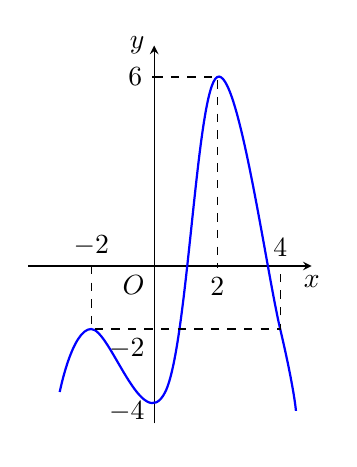
\begin{tikzpicture}[>=stealth,x=1.0cm,y=1.0cm,scale=0.4]
			\draw[->] (-4,0) -- (5,0) node[below] {$x$};
			\draw[->] (0,-5) -- (0,7) node[left] {$y$};
			\foreach \x in {2}
			\draw[shift={(\x,0)},color=black] (0pt,2pt)--(0pt,-2pt) node[below] {$\x$};
			\foreach \y in {6}
			\draw[shift={(0,\y)},color=black] (2pt,0pt)--(-2pt,0pt) node[left] {$\y$};
			\draw (0,0) node[below left] {$O$} (-2,0) node[above]{$-2$} (4,0) node[above]{$4$} (0,-4) node[below left]{$-4$} (0,-2) node[below left]{$-2$};
			\draw[thick,blue] plot[smooth,tension=.65] coordinates{(-3,-4) (-2,-2) (0.35,-4) (2,6) (4,-2) (4.5,-4.6)};
			\draw[dashed] (-2,0)--(-2,-2)--(4,-2)--(4,0)  (0,6)--(2,6)--(2,0);
	\end{tikzpicture}}
	\loigiai{
		Hàm số đồng biến trên khoảng $(0; 2)$.
	}
\end{ex}

\begin{ex}%[0D3Y2-3]%[Dự án đề kiểm tra HKII NH22-23- Don Lee]%[Sở Hà Nam]
	Tìm tọa độ đỉnh của parabol $(P)\colon x^{2}-4x-3$.
	\choice
	{\True $(2;-7)$}
	{$(-1; 2)$}
	{$(-2; 9)$}
	{$(4;-15)$}
	\loigiai{
		Tọa độ đỉnh của parabol $(P)\colon x^{2}-4x-3$ là $I(2;-7)$.
	}
\end{ex}

\begin{ex}%[0D4B2-1]%[Dự án đề kiểm tra HKII NH22-23- Don Lee]%[Sở Hà Nam]
	Bất phương trình $2x^{2}-5x-3 \leq 0$ có tập nghiệm là
	\choice
	{$\left[-\dfrac{1}{3}; 2\right]$}
	{$\left[\dfrac{1}{2}; 3\right]$}
	{$\left[-3;-\dfrac{1}{2}\right]$}
	{\True $\left[-\dfrac{1}{2}; 3\right]$}
	\loigiai{
		Ta có $2x^{2}-5x-3 \leq 0 \Leftrightarrow -\dfrac{1}{2}\le x\le 3$.
	}
\end{ex}

\begin{ex}%[0D2Y2-2]%[Dự án đề kiểm tra HKII NH22-23- Don Lee]%[Sở Hà Nam]
	Miền nghiệm của hệ bất phương trình $\heva{&y\geq 0\\&x+y\geq 2\\&x+y\leq 4\\&-x+y \leq 2}$ chứa điểm nào dưới đây?
	\choice
	{$\left(\dfrac{5}{2}; 3\right)$}
	{$(2; 4)$}
	{$(3;-1)$}
	{\True $\left(\dfrac{1}{2}; 2\right)$}
	\loigiai{
		Ta có $x=\dfrac{1}{2}$; $y=2$ thỏa mãn hệ bất phương trình.
	}
\end{ex}

\begin{ex}%[0H2B3-2]%[Dự án đề kiểm tra HKII NH22-23- Don Lee]%[Sở Hà Nam]
	Cho đoạn thẳng $AB$ có trung điểm $I$. Gọi $N$ là trung điểm của đoạn $IA$. Khẳng định nào dưới đây đúng?
	\choice
	{$3\overrightarrow{AN}+\overrightarrow{NB}=\overrightarrow{0}$}
	{\True $3\overrightarrow{AN}+\overrightarrow{BN}=\overrightarrow{0}$}
	{$3\overrightarrow{NA}+\overrightarrow{BN}=\overrightarrow{0}$}
	{$\overrightarrow{AN}+3 \overrightarrow{BN}=\overrightarrow{0}$}
	\loigiai{
		Ta có $\overrightarrow{0}=\overrightarrow{AI}+\overrightarrow{BI}=2\overrightarrow{AN}+\overrightarrow{BN}+\overrightarrow{NI}=2\overrightarrow{AN}+\overrightarrow{BN}+\overrightarrow{AN}=3\overrightarrow{AN}+\overrightarrow{BN}$.
	}
\end{ex}

\begin{ex}% [0H1B3-1]%[Dự án đề kiểm tra HKII NH22-23- Don Lee]%[Sở Hà Nam]
	Cho tam giác $ABC$ có $AB=2$, $AC=4$ và $\widehat{A}=60^{\circ}$. Tính độ dài cạnh $BC$.
	\choice
	{\True $2\sqrt{3}$}
	{$3\sqrt{2}$}
	{$3$}
	{$2\sqrt{0}$}
	\loigiai{
		Ta có $BC^2=AB^2+AC^2-2\cdot AB\cdot AC\cdot \cos\widehat{A}=4+16-2\cdot 2\cdot 4\cdot \dfrac{1}{2}=12$.\\
		Suy ra $BC=2\sqrt{3}$.
	}
\end{ex}

\begin{ex}%[0H2B4-1]%[Dự án đề kiểm tra HKII NH22-23- Don Lee]%[Sở Hà Nam]
	Cho tam giác $ABC$ vuông cân tại $A$ và $AB=2$. Tính $\overrightarrow{CB} \cdot \overrightarrow{BA}$.
	\choice
	{$-4\sqrt{2}$}
	{$4$}
	{$4\sqrt{2}$}
	{\True $-4$} 
	\loigiai{
		Ta có $\overrightarrow{CB} \cdot \overrightarrow{BA}=\overrightarrow{BC} \cdot \overrightarrow{AB}=\left(\overrightarrow{AC}-\overrightarrow{AB}\right)\cdot \overrightarrow{AB}=\overrightarrow{AC}\cdot \overrightarrow{AB}-\overrightarrow{AB}^2=-AB^2=-4$.
	}
\end{ex}

\begin{ex}%[0H2B3-5]%[Dự án đề kiểm tra HKII NH22-23- Don Lee]%[Sở Hà Nam]
	Cho tam giác $ABC$ có trọng tâm $G$. Biểu diễn $\overrightarrow{BG}$ theo hai véc-tơ $\overrightarrow{BA}$, $\overrightarrow{BC}$ được kết quả là
	\choice
	{$\overrightarrow{BG}=\dfrac{2}{3}\overleftrightarrow{BA}+\dfrac{1}{3}\overrightarrow{BC}$}
	{$\overrightarrow{BG}=\dfrac{1}{3}\overrightarrow{BA}+\dfrac{2}{3}\overrightarrow{BC}$}
	{\True $\overrightarrow{BG}=\dfrac{1}{3}\left(\overrightarrow{BA}+\overrightarrow{BC}\right)$}
	{$\overrightarrow{BG}=\dfrac{2}{3}\left(\overrightarrow{BA}+\overrightarrow{BC}\right)$}
	\loigiai{
		Gọi $M$ là trung điểm của cạnh $AC$.\\
		Ta có $\overrightarrow{BG}=\dfrac{2}{3}\overrightarrow{BM}=\dfrac{2}{3}\cdot\dfrac{1}{2}\left(\overrightarrow{BA}+\overrightarrow{BC}\right)=\dfrac{1}{3}\left(\overrightarrow{BA}+\overrightarrow{BC}\right)$.
	}
\end{ex}

\begin{ex}% [0H2B4-1]%[Dự án đề kiểm tra HKII NH22-23- Don Lee]%[Sở Hà Nam]
	Cho các véc-tơ $\vec{a}$, $\vec{b}$ thỏa mãn $\left|\vec{a}\right|=1$, $\left|\vec{b}\right|=2$, $\left|\vec{a}+\vec{b}\right|=3$. Tích $\vec{a} \cdot \vec{b}$ bằng
	\choice
	{$-1$}
	{\True $2$}
	{$-2$}
	{$3$}
	\loigiai{
		\allowdisplaybreaks
		$\begin{aligned}[t]
			\text{Ta có} \quad 3^2&=\left|\vec{a}+\vec{b}\right|^2=\left(\vec{a}+\vec{b}\right)^2=\vec{a}^2+\vec{b}^2+2\cdot\vec{a} \cdot \vec{b}=\left|\vec{a}\right|^2+\left|\vec{b}\right|^2+2\cdot\vec{a} \cdot \vec{b}\\
			&=1^2+2^2+2\cdot\vec{a} \cdot \vec{b}
		\end{aligned}$\\
	$\Leftrightarrow 2\vec{a} \cdot \vec{b}=9-5=4 \Leftrightarrow \vec{a} \cdot \vec{b}=2$.
	}
\end{ex}

\begin{ex}%[0H2B4-3]%[Dự án đề kiểm tra HKII NH22-23- Don Lee]%[Sở Hà Nam]
	Cho hình vuông $ABCD$ có cạnh bằng $a$. Tính $\left|\overrightarrow{BA}-\overrightarrow{BC}+\overrightarrow{DC}\right|$.
	\choice
	{$2a$}
	{$a\sqrt{2}$}
	{\True $a$}
	{$0$}
	\loigiai{
		Ta có $\left|\overrightarrow{BA}-\overrightarrow{BC}+\overrightarrow{DC}\right|=\left|\overrightarrow{CA}+\overrightarrow{DC}\right|=\left|\overrightarrow{DA}\right|=a$.
	}
\end{ex}

\Closesolutionfile{ans}
%\begin{center}
%	\textbf{ĐÁP ÁN}
%	\inputansbox{10}{ans/ans}	
%\end{center}
\begin{center}
	\textbf{PHẦN 2 - TỰ LUẬN}
\end{center}
\begin{bt}%[0T3B2-4]%[Dự án đề kiểm tra HKII NH22-23- Nguyễn Cường%[Sở GD-ĐT Hà Nam]
	Cho hàm số $y=3x^2-6x-9$.
	\begin{enumerate}
		\item Chỉ ra khoảng đồng biến, khoảng nghịch biến của hàm số.
		\item Xác định tọa độ đỉnh và giao điểm của đồ thị hàm số với trục hoành.
	\end{enumerate}
	\loigiai{
		\begin{enumerate}
			\item Chỉ ra khoảng đồng biến, khoảng nghịch biến của hàm số.\\
			Tập xác định $\mathscr{D}=\mathbb{R}$.\\
			Tọa độ đỉnh của parabol là $I(1;-12)$.\\
			Bảng biến thiên
			\begin{center}
			
\begin{tikzpicture}[font=\footnotesize, line join=round, line cap=round, >=stealth,scale=1]
				\tkzTabInit[lgt=1.2,espcl=4]
				{$x$/1,$y$/2}
				{$-\infty$,$1$,$+\infty$}
				\tkzTabVar{+/$+\infty$,-/$-12$,+/$+\infty$}
			\end{tikzpicture}
		
			\end{center}
			Hàm số đồng biến trên khoảng $(1;+\infty)$.\\
			Hàm số nghịch biến trên khoảng $(-\infty;1)$.
			\item Xác định tọa độ đỉnh và giao điểm của đồ thị hàm số với trục hoành.\\
			Tọa độ đỉnh của parabol là $I(1;-12)$.\\
			Xét phương trình hoành độ giao điểm của đồ thị hàm số và trục hoành
			$$3x^2-6x-9=0\Leftrightarrow \hoac{&x=-1\\&x=3.}$$
			Vậy tọa độ giao điểm của đồ thị hàm số với trục hoành là $A(-1;0)$ và $B(3;0)$.
		\end{enumerate}
	}
\end{bt}
\begin{bt}%[0T5K3-5]%[Dự án đề kiểm tra HKII NH22-23- Nguyễn Cường%[Sở GD-ĐT Hà Nam]
Cho tam giác $ABC$ có trọng tâm $G$. Gọi $I$ là trung điểm $AG$ và $M$, $N$ lần lượt là các điểm thỏa mãn $\overrightarrow{MN}=4\overrightarrow{MA}+\overrightarrow{MB}+\overrightarrow{MC}$. Chứng minh rằng ba điểm $M$, $I$, $N$ thẳng hàng.
\loigiai{
\immini
{
Ta có 
\allowdisplaybreaks
\begin{eqnarray*}
	\overrightarrow{MN}&=&4\overrightarrow{MA}+\overrightarrow{MB}+\overrightarrow{MC}\\
	&=&4\left(\overrightarrow{MI}+\overrightarrow{IA}\right)+\overrightarrow{MI}+\overrightarrow{IB}+\overrightarrow{MI}+\overrightarrow{IC}\\
	&=&6\overrightarrow{MI}+4\overrightarrow{IA}+\overrightarrow{IB}+\overrightarrow{IC}
\end{eqnarray*}
Gọi $D$ là trung điểm $BC$, ta có $\overrightarrow{IB}+\overrightarrow{IC}=2\overrightarrow{ID}$.\\
Mà $I$ là trung điểm $AG$ nên $\overrightarrow{ID}=2\overrightarrow{AI}$.\\
Do đó, $4\overrightarrow{IA}+\overrightarrow{IB}+\overrightarrow{IC}=4\overrightarrow{IA}+4\overrightarrow{AI}=\overrightarrow{0}$.\\
Suy ra $\overrightarrow{MN}=6\overrightarrow{MI}$, hay ba điểm $M$, $I$, $N$ thẳng hàng.
}
{
\begin{tikzpicture}[font=\footnotesize, line join=round, line cap=round, >=stealth,scale=1]
	\path (0:0) coordinate (B)
	+(0:5) coordinate (C)
	+(70:3) coordinate (A)
	($(B)!.5!(C)$)coordinate (D)
	($(A)!2/3!(D)$)coordinate (G)
	($(A)!.5!(G)$)coordinate (I)
	;
	\draw (A)--(B)--(C)--cycle
	;
	\draw[->](I)--(B);
	\draw[->](I)--(A);
	\draw[->](I)--(C);
	\draw[->](I)--(D);
	\foreach \x/\g in {B/180,C/0,A/90,D/-90,G/45,I/45}
	\fill (\x) circle (1pt)
	+(\g:3mm) node{$\x$};
\end{tikzpicture}

}
}
\end{bt}
\begin{bt}%[0T7K3-2]%[Dự án đề kiểm tra HKII NH22-23- Nguyễn Cường%[Sở GD-ĐT Hà Nam]
Giải các phương trình sau
	\begin{enumerate}
		\item $\sqrt{2x^2-2x+3}=\sqrt{x^2-8x-2}$;
		\item $\sqrt{5x^2-6x-4}=2(x-1)$.
	\end{enumerate}
	\loigiai{
		\begin{enumerate}
			\item Ta có
			\allowdisplaybreaks
			\begin{eqnarray*}
				\sqrt{2x^2-2x+3}=\sqrt{x^2-8x-2}&\Rightarrow&2x^2-2x+3=x^2-8x-2\\
				&\Leftrightarrow& x^2+6x+5=0\\
				&\Leftrightarrow&\hoac{&x=-1\\&x=-5.}
			\end{eqnarray*}
		\begin{itemize}
			\item Với $x=-1$ thế vào phương trình ban đầu ta có $\sqrt{7}=\sqrt{7}$ nên $x=-1$ là nghiệm của phương trình.
			\item Với $x=-5$ thế vào phương trình ban đầu ta có $3\sqrt{9}=3\sqrt{9}$ nên $x=-5$ là nghiệm của phương trình.
		\end{itemize}
	Vậy tập nghiệm của phương trình là $S=\{-5;-1\}$.
			\item Ta có
			\allowdisplaybreaks
			\begin{eqnarray*}
				\sqrt{5x^2-6x-4}=2(x-1)&\Rightarrow&5x^2-6x-4=4(x^2-2x+1)\\
				&\Leftrightarrow& x^2+2x-8=0\\
				&\Leftrightarrow&\hoac{&x=2\\&x=-4.}
			\end{eqnarray*}
			\begin{itemize}
				\item Với $x=2$ thế vào phương trình ban đầu ta có $\sqrt{4}=2$ nên $x=2$ là nghiệm của phương trình.
				\item Với $x=-4$ thế vào phương trình ban đầu ta có $\sqrt{100}=-10$ nên $x=-4$ là không nghiệm của phương trình.
			\end{itemize}
			Vậy tập nghiệm của phương trình là $S=\{2\}$.
		\end{enumerate}
	}
\end{bt}


\begin{bt}%[0H2G4-3]%[Dự án đề kiểm tra HKI NH22-23- NGUYỄN VĂN SƠN %[SGD HÀ NAM]
Cho tam giác đều $ABC$. Gọi $M$, $N$, $P$ lần lượt là các điểm thoả mãn\\ $\overrightarrow{BM}=k\overrightarrow{BC}$, $3\overrightarrow{AN}=2\overrightarrow{AB}$, $5\overrightarrow{AP}=2\overrightarrow{AC}.$\\
	\begin{enumerate}
		\item Biểu diễn $\overrightarrow{AM}$ theo hai véc-tơ $\overrightarrow{AB}$, $\overrightarrow{AC}$.\\
		\item Tìm $k$ để hai đường thẳng $AM$, $NP$ vuông góc với nhau.
	\end{enumerate}
\loigiai{
	
	\begin{enumerate}
	\item  Từ giả thiết $\overrightarrow{BM}=k\overrightarrow{BC}$ 
	$\Rightarrow \overrightarrow{AM}-\overrightarrow{AB}=k(\overrightarrow{AC}-\overrightarrow{AB})$ $\Rightarrow  \overrightarrow{AM}=(1-k) \overrightarrow{AB}+k\overrightarrow{AC}$.
	\item Theo giả thiết $3\overrightarrow{AN}=2\overrightarrow{AB} \Rightarrow$ $3(\overrightarrow{AP}+\overrightarrow{PN})=2\overrightarrow{AB}$$\Rightarrow$ $ 3\overrightarrow{PN}=2\overrightarrow{AB}-3\overrightarrow{AP} \quad $ (1).\\
	Mặt khác $5\overrightarrow{AP}=2\overrightarrow{AC}$$\Rightarrow$$\overrightarrow{AP}=\dfrac{2}{5}\overrightarrow{AC}\quad $ (2).\\
	Từ (1) và (2) ta có: $ \overrightarrow{PN}=\dfrac{2}{3}\overrightarrow{AB}-\dfrac{2}{5}\overrightarrow{AC}$.\\
	Để $AM$ và $NP$ vuông góc với nhau thì $ \overrightarrow{AM}.\overrightarrow{PN}=0$\\
	$\Leftrightarrow \left((1-k)\overrightarrow{AB}+k\overrightarrow{AC}\right)\left( \dfrac{2}{3}\overrightarrow{AB}-\dfrac{6}{5}\overrightarrow{AC}\right)=0$\quad (*).\\
	Đặt $AB=AC=BC=a$. Khi đó ta có $\overrightarrow{AB}.\overrightarrow{AC} = \left| \overrightarrow{AB}\right|.\left| \overrightarrow{AC}\right|.\cos 60^\circ = \dfrac{a^2}{2}$. \\
	Từ (*) ta có $\dfrac{2(1-k)}{3}\cdot a^2-\dfrac{6(1-k)}{5}\cdot a^2.\dfrac{1}{2}+\dfrac{2k}{3}.a^2\cdot\dfrac{1}{2}-\dfrac{6k}{5}\cdot a^2=0$
	$\Rightarrow k=\dfrac{7}{8}$.	
	\end{enumerate}
}
\end{bt}
\begin{bt}%[0H1G3-2]%[Dự án đề kiểm tra HKI NH22-23- NGUYỄN VĂN SƠN %[SGD HÀ NAM]
	Anh Việt có một mảnh đất hình từ giác $ABCD$ với $AB=4{,}2$ m, $BC=15{,}3$ m, $CD=5{,}4$ m và $DA=16{,}8$ m. Để tính diện tích mảnh đất, anh Việt lấy các điểm $M$, $N$ lần lượt trên cạnh $AB, AD$ sao cho $AM=1$ m và $AN=1$ m. Anh việt đo được $MN=1{,}7$ m. Tính diện tích mảnh đất (làm tròn kết quả đến hàng phần trăm).
	
	\loigiai{
		\begin{center}
			\begin{tikzpicture}[scale=0.7, font=\footnotesize,>=stealth]
				%Định nghĩa điểm.
				\coordinate (A) at (1,4);
				\coordinate (B) at (0,0);
				\coordinate (C) at (13,0);
				\coordinate (D) at (14,6);
				%Vẽ tứ giác ABCD.
				\draw (A)--(B)--(C)--(D)--cycle;
				\coordinate (M) at ($(A)!0.1!(D)$);
				\coordinate (N) at ($(A)!0.3!(B)$);
				\draw (D)--(B) (M)--(N);
				%Hiển thị các điểm.
				\foreach \x/\y in {A/150,B/180,C/0,D/90,M/90, N/150}{\fill (\x) circle(2pt) ($(\x)+(\y:0.3cm)$) node{$\x$};}
			\end{tikzpicture}
		\end{center}
		\begin{itemize}
			\item Xét tam giác $AMN$, ta có
			\begin{eqnarray*}
				&&MN^2=AM^2+AN^2-2\cdot AM \cdot AN \cdot \cos A\\
				&\Leftrightarrow& (1{,}7)^2=1^2+1^2-2\cdot 5\cdot 1\cdot \cos A\\
				&\Leftrightarrow& \cos A=-\dfrac{89}{200}.
			\end{eqnarray*}
			\item Xét tam giác $ABD$, ta có
			\begin{eqnarray*}
				&&BD^2=AD^2+AB^2-2\cdot AB \cdot AD \cdot \cos A\\
				&\Leftrightarrow& BD^2=(4{,}2)^2+(16{,}8)^2-2\cdot (4{,}2)^2\cdot (16{,}8)^2\cdot\dfrac{-89}{200} \\
				&\Leftrightarrow& BD \approx 19{,}05.
			\end{eqnarray*}
			\item Tính diện tích tam giác $ABD$, ta có
			$p=\dfrac{AB+AD+BD}{2}$.\\
			Suy ra
			\begin{eqnarray*}
				S_{\triangle ABD}&=&\sqrt{p(p-AB)(p-AD)(p-BD)}\\
				&=&\sqrt{p(p-4{,}2)(p-16{,}8)(p-19{,}05)}\approx 31{,}59\, \text{m}^2.
			\end{eqnarray*}
			
			\item Tương tự, tính diện tích tam giác $BCD$, ta có
			$p=\dfrac{BC+BD+CD}{2}$.\\
			Suy ra 
			\begin{eqnarray*}
				S_{\triangle BCD}&=&\sqrt{p(p-BC)(p-CD)(p-BD)}\\
				&=&\sqrt{p(p-15{,}3)(p-5{,}4)(p-19{,}05)}\approx 32{,}99\, \text{m}^2.
			\end{eqnarray*}
			
			\item Vậy $S_{ABCD}=S_{\triangle ABD}+S_{\triangle BCD}\approx 64{,}58$ m$^2$.
		\end{itemize}
	}
\end{bt}
\begin{bt}%[0D3G1-6] %[Dự án đề kiểm tra HKI NH22-23- NGUYỄN VĂN SƠN %[SGD HÀ NAM]
	Một quán cà phê đang bán ở mức giá $7000$ đồng cho mỗi cốc cà phê, trung bình mỗi tháng quán bán được $3900$ cốc. Chủ quán muốn tăng giá bán để thêm doanh thu, biết rằng nếu mỗi cốc cà phê cứ tăng thêm $1000$ đồng thì số cốc bán được trung bình mỗi tháng lại giảm đi $300$. Hỏi chủ quán phải bán với mức giá bao nhiêu một cốc cà phê để doanh thu của quán trong tháng là cao nhất?
	\loigiai
	{
		Gọi số tiền cần tăng là $x$ (nghìn đồng).\\
		Mỗi lần tăng $x$ (nghìn đồng) thì số cốc trung bình mỗi tháng lại giảm đi $300x$.\\
		Doanh thu mỗi tháng của cửa hàng là\\
		 $f(x)=(7+x)(3900-300x)=-300x^2+1800x+27300=-300(x-3)^2+30000 \le 30000$.\\
		Doanh thu của quán trong tháng cao nhất khi $f(x)$ đạt giá trị lớn nhất.\\
		Suy ra doanh thu của quán trong tháng cao nhất là $30000$ khi giá tăng là $3$ (nghìn đồng) và chủ quán phải bán với giá $3000 + 7000 = 10000$ đồng.
		
}
\end{bt}




